
\documentclass[a4paper,conference]{IEEEtran}

\usepackage{color}
\usepackage{amsmath}
\usepackage{algorithm}
\usepackage{algorithmic}
\usepackage{threeparttable}
\usepackage[normalem]{ulem}

\usepackage[colorinlistoftodos]{todonotes}

\ifCLASSINFOpdf
\else
\fi

\hyphenation{}


\begin{document}

\title{\textcolor{blue}{Evaluating Prediction Quality 
without Ground Truth}}

\author{\IEEEauthorblockN{Dheeraj Bhaskaruni}
\IEEEauthorblockA{\textcolor{blue}{Department of Computer Science}\\
University of Wyoming\\
Laramie, Wyoming - 82070\\
Email: vbhaskar@uwyo.edu}
\and
\IEEEauthorblockN{Chao Lan}
\IEEEauthorblockA{Department of Computer Science\\
University of Wyoming \\ 
Laramie, Wyoming, 82070\\
Email: clan@uwyo.edu} 
}

\maketitle

\begin{abstract}
\textcolor{blue}{
In academic research, to evaluate prediction quality of 
machine learning models, it is typically assumed testing 
sample is labeled. However, this ground truth is not always 
available in practice, where testing instances are collected 
with way higher velocity than one can manually label them. 
How to evaluate a model's prediction error on unlabeled 
testing sample? This is the question we aim to address in this paper. 
}

\textcolor{blue}{
In this paper, we a measure of a model's prediction quality on 
unlabeled testing sample, presuming training
sample is labeled and training and testing sample distributions are 
identical; the measured quality include accuracy and f1 score. 
Given a testing sample labeled by a model, our measure is the 
prediction quality on training sample given by the same model 
yet retrained on the labeled testing sample. 
Currently, the proposed measure remains heuristic, but we empirically 
show it is a more accurate estimate of prediction quality on testing 
sample than traditional estimate based solely on training sample; 
we also discuss its 
connection to self-taught learning which partly motivates 
the present study. 
}

\sout{
In this paper, we propose an evaluation method to predict model accuracy when there is no ground truth. Ideally when we predict the labels of test data, accuracy of the prediction is calculated by comparing the predicted data with ground truth.Most studies assume ground truth is known for testing data, but in reality if it is unknown there is no well documented way of predicting accuracy. We evaluate the method proposed to calculate the accuracy and F1-Score for a any dataset (in this case we have used kaggle malware dataset). }
\end{abstract}


\IEEEpeerreviewmaketitle



\section{Introduction}

\textcolor{red}{don't worry about it for now}

\textcolor{red}{1. describe what's the problem with common 
evaluation approach? assume ground truth, but often not available}

\textcolor{red}{2. describe how people address this problem? 
basically they can't, but they use some approximate estimate 
such as training error. why this is bad?}

\textcolor{red}{3. describe another line of research that motivates 
your idea? (multi-view learning? self-taught learning?)}

\textcolor{red}{4. describe your proposed idea}


\textcolor{red}{5. describe your experimental studies and results}


\textcolor{red}{6. describe the organization of your study}


\section{\textcolor{blue}{The Proposed Measure of Prediction Quality}} 

\textcolor{blue}{In this section, we present the proposed 
measure of prediction quality on unlabeled testing sample.} 

\textcolor{red}{ First introduce any notation you are going to use 
and explain the problem setting, e.g. we assume a training 
set is labeled, and a testing set is not labeled, etc}

We assume that the training set is labeled (because this is data from the past) and testing set is unlabeled (since this data is fairly new and hence unclassified). We also assume that the training set and testing set is almost identical.


\textcolor{red}{then explain your evaluation approach. you can put it 
in an algorithm framework} 

\begin{algorithm}[t!]
\begin{algorithmic}
   \STATE {\bfseries Input:} Train set (fully labeled), Test set (partially labeled/unlabeled)\\   
   \FOR {for loop?}
   	   \STATE 1: 
       \STATE 2:
	   \STATE 3: 
   \ENDFOR
   \vskip -0.2in
\end{algorithmic}
   \caption{Evaluation Approach}
\label{alg1}
\end{algorithm}

\textcolor{red}{now argue why do you think this is a 
good estimate (intuitively) e.g. if training and testing 
distributions are identical, it should be good. }

In the above algorithm it is very clear that we are predicting the model accuracy based on the training and testing accuracies. This will be a good estimate only when the training set and testing set are have equally distributed similar data. If they are not similar then we cannot compare both the accuracies from forward and backward passes to identify a metric to measure the model accuracy.

\textcolor{red}{Also explain how do you plan to evaluate 
distribution difference? Give mathematical formula}

The similarity in the distributions of train and test sets is measured using a well defined method which is called Z-test. It is used for comparing two samples directly, we can compute the Z statistic in the following manner:

\[ Z = \frac{(\overline{X_1} - \overline{X_2})}{\sqrt{\sigma^2_{X_1} - \sigma^2_{X_2}}} \]
Here, in the above formula
\begin{description}
\item[$\ast$]$\overline{X_1}$ is the mean value of training set
\item[$\ast$]$\overline{X_2}$ is the mean value of test set
\item[$\ast$]$\sigma_{X_1}$ is the standard deviation of training set divided by the square root of the number of data points
\item[$\ast$]$\sigma_{X_2}$ is the standard deviation of test set divided by the square root of the number of data points
\end{description}
\textcolor{red}{finally, discuss what inspired you of 
this idea? multi-view leraning? self-taught learning?
what can be the connections? (Don't worry much about 
this part for now)} 

Once we have the Z-statistic calculated from above we can use the same to predict the similarity of the two data distributions

\begin{description}
\item[$\ast$]If the Z-statistic is less than 2, the two samples are the same. 
\item[$\ast$]If the Z-statistic is between 2.0 and 2.5, the two samples are marginally different 
\item[$\ast$]If the Z-statistic is between 2.5 and 3.0, the two samples are significantly different 
\item[$\ast$]If the Z-statistic is more then 3.0, the two samples are highly signficantly different
\end{description}

In our case for the malware dataset we have considered the Z-statistic is well below 2 which implies the train and test sets are fairly identically distributed.

Final Z-Score calculated for malware train and test dataset is: 0.0012 $<<$ 2, which means there is no significant difference between  train and test sets which implies the data distribution in train and test sets is identical.
\begin{table}[t!]
\renewcommand{\arraystretch}{1.3} 
\caption{Z Statistic measure calculation of KAGGLE Malware Datset}
\centering
\begin{threeparttable}
\begin{tabular}{lll} %
\bf Training/Testing & \bf Metric & \bf Value \\ \hline 
Training & $\overline{X_1}$ or Mean & 60026.0007 \\ 
Training & Standard Deviation & 1844375.6061 \\ 
Training & $\sigma_{X_1}$$^{(*)}$ & 17691.9032 \\ 
Testing & $\overline{X_2}$ or Mean & 58265.8489 \\ 
Testing & Standard Deviation & 1748762.6902 \\ 
Testing & $\sigma_{X_2}$$^{(+)}$ & 16774.7502 \\ 
\end{tabular}
\begin{tablenotes}
\item[$(\ast)$]$\sigma_{X_1}$ is calculated using the standard deviation of training set
\item[$(+)$]$\sigma_{X_2}$ is calculated using the standard deviation of test set
\end{tablenotes}
\end{threeparttable}
\end{table}

\section{Experiment}

\textcolor{blue}{In this section, we empirically evaluate the 
proposed measure on a real-world data set.}

\subsection{Dataset Description}

\textcolor{red}{verbally describe your data set, what is the task, 
what are features, etc; don't just give a table}

\textcolor{red}{first describe the original data set, then describe 
how you preprocessed it} 

\textcolor{red}{when describing what you did in experiments, 
use past tense} 


In this section, we \textcolor{blue}{describe the data set used 
in experiments}. \sout{discuss the basic details of the dataset used by method applied in this paper. In order to show and depict accuracy of our proposed method we have used the data from BIG MALWARE CLASSIFICATION CHALLENGE 2015 of KAGGLE.} 
\textcolor{blue}{We collected the Big Malware classification Challenge 2015 data set from Kaggle}.\textcolor{red}{give a reference or link for 
the data set}. 
\textcolor{blue}{The data set contains XX} 
\textcolor{red}{give an exact number}
\textcolor{blue}{malwares categorized 
into 9 classes, including...... Malwares are described by 230 features,
including bag-of-words, ....... For detailed information, please refer 
to (the original website of the data set)}
\textcolor{red}{I assume there are text information in 
malware? clarify}. 
\textcolor{blue}{The machine learning task is to classify malwares 
into 9 classes based on their features.} 
\textcolor{red}{now describe how you preprocessed the data set; 
for instance, why do you downsample the data set?} 
\textcolor{blue}{For computational efficiency, we (randomly?) 
downsampled the data set to 10,000 instances.}


\textcolor{red}{How did you split data into training and testing? 
clarify here...} 


\begin{description}
\item[$\ast$] \sout{10868 instances (originally there are around 20,000 instances but we have only considered around 10,000 instances)}
\item[$\ast$] \sout{230 features + 1 Label which holds malware category}
\item[$\ast$] \sout{9 classes}
\end{description}


\sout{The proposed method Backward Evaluation Data Training estimates the model accuracy of a classification task. All the features that we have in this dataset are numerical features.}

\sout{The features have been extracted from the malware files. All the features are extracted using many data extraction techniques like} 
\begin{description}
\item[$\ast$] \sout{Bag of Words}
\item[$\ast$] \sout{BigGrams}
\item[$\ast$] \sout{1-Grams}
\item[$\ast$] \sout{Size Of File}
\end{description}
\sout{applied on the instructions in the malware files}.

\sout{There is no missing data as well as there are no categorical features in this dataset. Methods implemented in this project are all off-line techniques}

\subsection{Assumptions for Backward Evaluation Data Training}
In this paper we make an important assumption that is going into this project. We assume that the distribution and frequency of labels in both train and test sets to be identical.

In order to support our assumption we applied z-test and found that the data present in train and test datasets is very identical and hence can be used for our experiment.

%\begin{figure}[h]
%\centering
%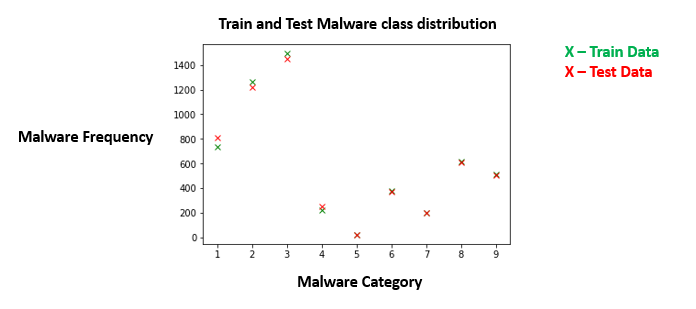
\includegraphics[width=2.5\textwidth]{Data_Distribution.PNG}
%\DeclareGraphicsExtensions
%\caption{Simulation results for the network.}
%\label{fig_sim}
%\end{figure}

\subsection{Metrics and Terms used in Backward Evaluation Data Training}
\begin{enumerate}
\item Training Accuracy: The accuracy calculated in the forward pass by comparing the predicted test labels with the test data ground truth. We use ground truth to show the accuracy of the Backward Evaluation Data Training method.
\item Re-Training Accuracy: The accuracy calculated in the backward pass by training the model on the newly predicted test data and predicting the training labels and comparing it to the train data ground truth.

Then we compare training accuracy and re-training accuracy to identify a metric to find a measure to predict the model accuracy when there is no ground truth.
\end{enumerate}
\subsection{Backward Evaluation Data Training Method}
We implement this method few detailed steps
\begin{enumerate}
\item We predict the labels of unlabeled test data without any prior knowledge using model f1
\item We train the model f2 on the test instances and previously predicted test labels and predict training instances
\item Calculate the prediction accuracy using the ground truth of train data and predicted train labels
\item Also calculate the accuracy of the prior predicted test data without prior knowledge comparing it with test data ground truth, this is only for validating the result of our method
\item If both the accuracies calculated above are similar, it implies that the Backward Evaluation Data Training method is accurate
\end{enumerate}

%\begin{figure}[h]
%\centering
%\includegraphics[width=.25\textwidth]{Backward_data_training.PNG} 
%\caption{Backward data evaluation Training}
%\end{figure}

\subsection{Results for Back-Forth Data Training}
Refer TABLE II for proposed method accuracy comparison with training and testing accuracies
and TABLE III for proposed method F1-Score comparison with training and testing F1-Scores.
\begin{table}[t!]
\renewcommand{\arraystretch}{1.3} 
\caption{Proposed Model Accuracy Comparison}
\centering
\begin{threeparttable}
\begin{tabular}{llllll} %
\bf Model Name & \bf Training & \bf Testing & \bf Proposed & \bf Difference$^1$ & \bf Difference$^2$  \\ \hline 
Linear & 0.2664 & 0.2712 & 0.2703 & 0.00482 &  0.00092\\ 
Ridge  & 0.9449 & 0.8303 & 0.7887 & 0.11475 & 0.04159\\
Naive Bayes  & 0.79094  & 0.39694 & 0.36658 & 0.39000 & 0.03036\\
Decision Tree & 1.0000 & 0.9705 & 0.9740 & 0.02958 & 0.00350\\ 
Random Forest & 0.9900 & 0.9830 & 0.9804 & 0.00727 & 0.00258\\ 
\end{tabular}
\begin{tablenotes}
\item[1]Difference is the absolute difference between testing accuracy and training accuracy
\item[2]Difference is the absolute difference between testing accuracy and proposed accuracy metric
\end{tablenotes}
\end{threeparttable}
\end{table}


\begin{table}[t!]
\renewcommand{\arraystretch}{1.3} 
\caption{Proposed Model F1-Score Comparison}
\centering
\begin{threeparttable}
\begin{tabular}{llllll} %
\bf Model Name & \bf Training & \bf Testing & \bf Proposed & \bf Difference$^1$ & \bf Difference$^2$  \\ \hline 
Linear & 0.1121 & 0.1157 & 0.1150 & 0.00362 & 0.00070\\ 
Ridge  & 0.9444  & 0.8239 & 0.7769 & 0.12056 & 0.04700\\
Naive Bayes  & 0.78563  & 0.34120 & 0.30951 & 0.44443 & 0.03169\\
Decision Tree & 1.0000 & 0.9702 & 0.9739 & 0.02987 & 0.00375\\ 
Random Forest & 0.9900 & 0.9828 & 0.9803 & 0.00721 & 0.00252\\ 
\end{tabular}
\begin{tablenotes}
\item[1]Difference is the difference between testing F1-score and training F1-score
\item[2]Difference is the difference between testing F1-score and proposed F1-score metric
\end{tablenotes}
\end{threeparttable}
\end{table}
% An example of a floating figure using the graphicx package.
% Note that \label must occur AFTER (or within) \caption.
% For figures, \caption should occur after the \includegraphics.
% Note that IEEEtran v1.7 and later has special internal code that
% is designed to preserve the operation of \label within \caption
% even when the captionsoff option is in effect. However, because
% of issues like this, it may be the safest practice to put all your
% \label just after \caption rather than within \caption{}.
%
% Reminder: the "draftcls" or "draftclsnofoot", not "draft", class
% option should be used if it is desired that the figures are to be
% displayed while in draft mode.
%
%\begin{figure}[!t]
%\centering
%\includegraphics[width=2.5in]{myfigure}
% where an .eps filename suffix will be assumed under latex,
% and a .pdf suffix will be assumed for pdflatex; or what has been declared
% via \DeclareGraphicsExtensions.
%\caption{Simulation results for the network.}
%\label{fig_sim}
%\end{figure}

% Note that the IEEE typically puts floats only at the top, even when this
% results in a large percentage of a column being occupied by floats.


% An example of a double column floating figure using two subfigures.
% (The subfig.sty package must be loaded for this to work.)
% The subfigure \label commands are set within each subfloat command,
% and the \label for the overall figure must come after \caption.
% \hfil is used as a separator to get equal spacing.
% Watch out that the combined width of all the subfigures on a
% line do not exceed the text width or a line break will occur.
%
%\begin{figure*}[!t]
%\centering
%\subfloat[Case I]{\includegraphics[width=2.5in]{box}%
%\label{fig_first_case}}
%\hfil
%\subfloat[Case II]{\includegraphics[width=2.5in]{box}%
%\label{fig_second_case}}
%\caption{Simulation results for the network.}
%\label{fig_sim}
%\end{figure*}
%
% Note that often IEEE papers with subfigures do not employ subfigure
% captions (using the optional argument to \subfloat[]), but instead will
% reference/describe all of them (a), (b), etc., within the main caption.
% Be aware that for subfig.sty to generate the (a), (b), etc., subfigure
% labels, the optional argument to \subfloat must be present. If a
% subcaption is not desired, just leave its contents blank,
% e.g., \subfloat[].


% An example of a floating table. Note that, for IEEE style tables, the
% \caption command should come BEFORE the table and, given that table
% captions serve much like titles, are usually capitalized except for words
% such as a, an, and, as, at, but, by, for, in, nor, of, on, or, the, to
% and up, which are usually not capitalized unless they are the first or
% last word of the caption. Table text will default to \footnotesize as
% the IEEE normally uses this smaller font for tables.
% The \label must come after \caption as always.
%
%\begin{table}[!t]
%% increase table row spacing, adjust to taste
%\renewcommand{\arraystretch}{1.3}
% if using array.sty, it might be a good idea to tweak the value of
% \extrarowheight as needed to properly center the text within the cells
%\caption{An Example of a Table}
%\label{table_example}
%\centering
%% Some packages, such as MDW tools, offer better commands for making tables
%% than the plain LaTeX2e tabular which is used here.
%\begin{tabular}{|c||c|}
%\hline
%One & Two\\
%\hline
%Three & Four\\
%\hline
%\end{tabular}
%\end{table}


% Note that the IEEE does not put floats in the very first column
% - or typically anywhere on the first page for that matter. Also,
% in-text middle ("here") positioning is typically not used, but it
% is allowed and encouraged for Computer Society conferences (but
% not Computer Society journals). Most IEEE journals/conferences use
% top floats exclusively.
% Note that, LaTeX2e, unlike IEEE journals/conferences, places
% footnotes above bottom floats. This can be corrected via the
% \fnbelowfloat command of the stfloats package.




\section{Conclusion}
The conclusion goes here.




% conference papers do not normally have an appendix


% use section* for acknowledgment
%\section*{Acknowledgment}


%The authors would like to thank...





% trigger a \newpage just before the given reference
% number - used to balance the columns on the last page
% adjust value as needed - may need to be readjusted if
% the document is modified later
%\IEEEtriggeratref{8}
% The "triggered" command can be changed if desired:
%\IEEEtriggercmd{\enlargethispage{-5in}}

% references section

% can use a bibliography generated by BibTeX as a .bbl file
% BibTeX documentation can be easily obtained at:
% http://mirror.ctan.org/biblio/bibtex/contrib/doc/
% The IEEEtran BibTeX style support page is at:
% http://www.michaelshell.org/tex/ieeetran/bibtex/
%\bibliographystyle{IEEEtran}
% argument is your BibTeX string definitions and bibliography database(s)
%\bibliography{IEEEabrv,../bib/paper}
%
% <OR> manually copy in the resultant .bbl file
% set second argument of \begin to the number of references
% (used to reserve space for the reference number labels box)
\begin{thebibliography}{1}

\bibitem{IEEEhowto:kopka}
H.~Kopka and P.~W. Daly, \emph{A Guide to \LaTeX}, 3rd~ed.\hskip 1em plus
  0.5em minus 0.4em\relax Harlow, England: Addison-Wesley, 1999.

\end{thebibliography}




% that's all folks
\end{document}


